\documentclass{article}
\usepackage[T1]{fontenc}
\usepackage[scaled=0.94]{helvet}
\renewcommand{\familydefault}{\sfdefault}
\usepackage{tikz}
\usetikzlibrary{arrows.meta}
\pagestyle{empty}
\setlength{\parindent}{0pt}
\setlength{\topskip}{0pt}
\setlength{\parskip}{0pt}
\definecolor{ink}{HTML}{262B30}
\definecolor{bluew}{HTML}{356D96}
\definecolor{loserfill}{HTML}{D7DCE0}
\definecolor{loseredge}{HTML}{8E969C}
\definecolor{unreadfill}{HTML}{EEF1F3}
\definecolor{unreadt}{HTML}{9BA3AA}
\definecolor{edgec}{HTML}{AAB1B7}
\definecolor{edgepale}{HTML}{D8DEE2}
\definecolor{ptrc}{HTML}{303840}
\definecolor{exh}{HTML}{C44C3C}
\definecolor{muted}{HTML}{6E777E}
\definecolor{container}{HTML}{C5CCD1}
\definecolor{containerpale}{HTML}{E1E5E8}
\definecolor{palebg}{HTML}{F7F8F9}
\definecolor{gapbg}{HTML}{FBFCFC}
\definecolor{white}{HTML}{FFFFFF}
\newcommand{\numfont}{\sffamily\bfseries\fontsize{6.15}{7}\selectfont}
\newcommand{\labelfont}{\sffamily\fontsize{5.7}{6.6}\selectfont}
\newcommand{\captionfont}{\sffamily\fontsize{6.05}{7.1}\selectfont}
\newcommand{\idfont}{\sffamily\fontsize{6.35}{7.4}\selectfont}
\newcommand{\headfont}{\sffamily\bfseries\fontsize{8}{9.2}\selectfont}
\newcommand{\titlefont}{\sffamily\bfseries\fontsize{7.15}{8.3}\selectfont}
\begin{document}
\pdfhorigin=0bp
\pdfvorigin=0bp
\setbox0=\hbox{%
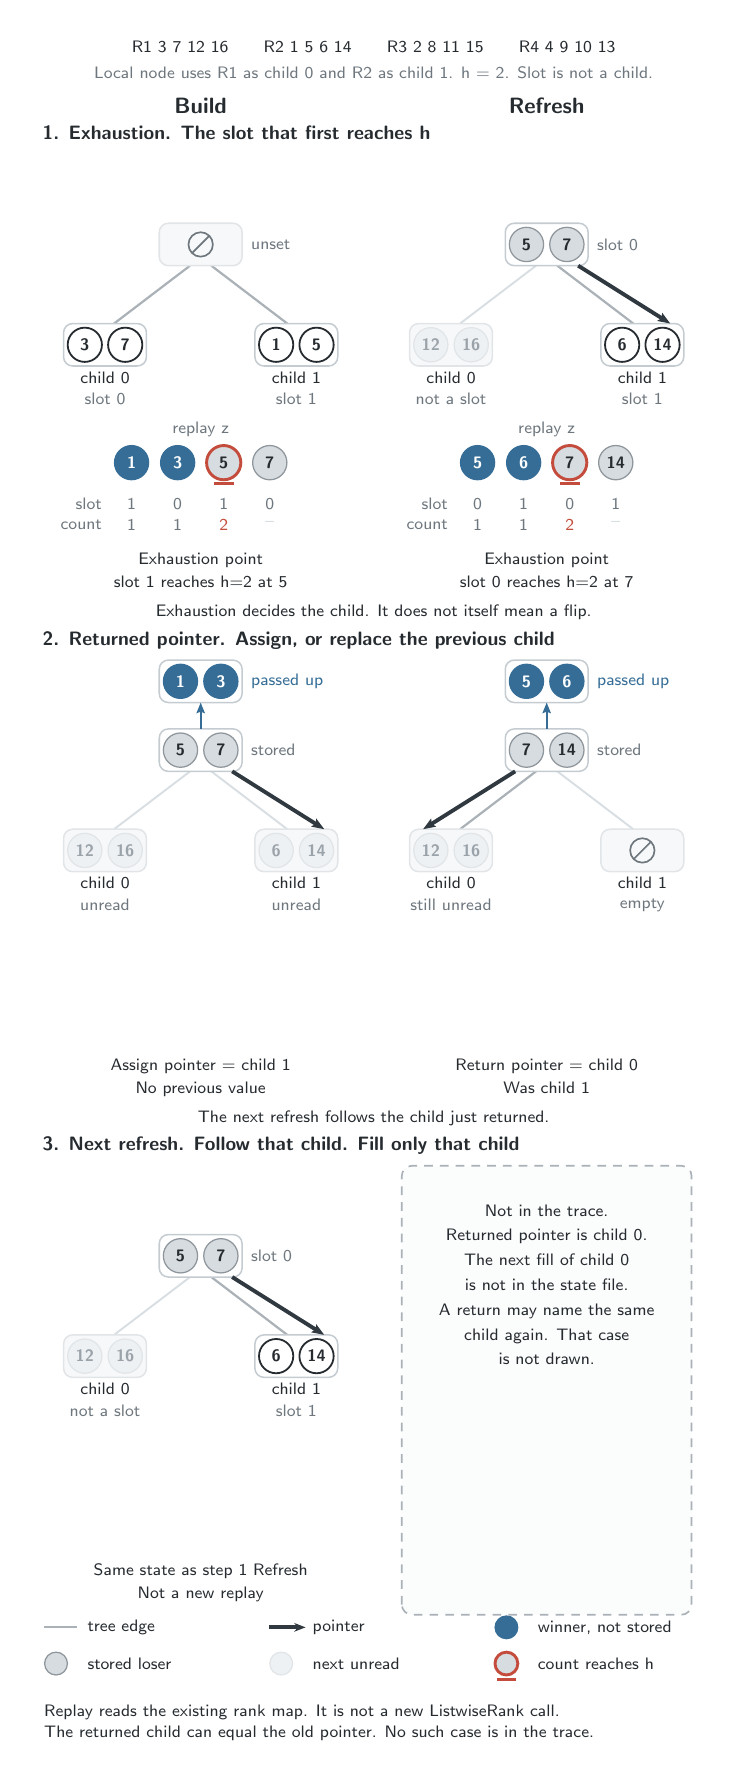
\begin{tikzpicture}[x=1mm,y=1mm,every node/.style={inner sep=0pt,outer sep=0pt}]
\node[inner sep=0pt, anchor=north, align=center, font=\idfont, text=ink] at (43.942,216.060) {R1  3 7 12 16\qquad R2  1 5 6 14\qquad R3  2 8 11 15\qquad R4  4 9 10 13};
\node[inner sep=0pt, anchor=north, align=center, font=\captionfont, text=muted] at (43.942,212.760) {Local node uses R1 as child 0 and R2 as child 1. h = 2. Slot is not a child.};
\node[inner sep=0pt, anchor=north, align=center, font=\headfont, text=ink] at (21.971,208.760) {Build};
\node[inner sep=0pt, anchor=north, align=center, font=\headfont, text=ink] at (65.913,208.760) {Refresh};
\node[inner sep=0pt, anchor=north west, align=left, font=\titlefont, text=ink] at (1.900,205.260) {1. Exhaustion. The slot that first reaches h};
\draw[line width=0.8pt, draw=edgec, line cap=butt] (20.621,187.530) -- (10.971,180.180);
\draw[line width=0.8pt, draw=edgec, line cap=butt] (23.321,187.530) -- (32.971,180.180);
\draw[rounded corners=1.150mm, line width=0.55pt, draw=containerpale, fill=palebg] (16.711,187.530) rectangle (27.231,192.920);
\draw[line width=0.6pt, draw=muted] (21.971,190.225) circle (1.550mm);
\draw[line width=0.6pt, draw=muted] (20.921,189.175) -- (23.021,191.275);
\node[inner sep=0pt, anchor=west, align=left, font=\labelfont, text=muted] at (28.381,190.225) {unset};
\draw[rounded corners=1.150mm, line width=0.55pt, draw=container, fill=white] (4.561,174.790) rectangle (15.081,180.180);
\draw[line width=0.65pt, draw=ink, fill=white] (7.256,177.485) circle (2.175mm);
\node[inner sep=0pt, font=\numfont, text=ink] at (7.256,177.485) {3};
\draw[line width=0.65pt, draw=ink, fill=white] (12.386,177.485) circle (2.175mm);
\node[inner sep=0pt, font=\numfont, text=ink] at (12.386,177.485) {7};
\draw[rounded corners=1.150mm, line width=0.55pt, draw=container, fill=white] (28.861,174.790) rectangle (39.381,180.180);
\draw[line width=0.65pt, draw=ink, fill=white] (31.556,177.485) circle (2.175mm);
\node[inner sep=0pt, font=\numfont, text=ink] at (31.556,177.485) {1};
\draw[line width=0.65pt, draw=ink, fill=white] (36.686,177.485) circle (2.175mm);
\node[inner sep=0pt, font=\numfont, text=ink] at (36.686,177.485) {5};
\node[inner sep=0pt, anchor=north, align=center, font=\labelfont, text=ink] at (9.821,174.090) {child 0};
\node[inner sep=0pt, anchor=north, align=center, font=\labelfont, text=muted] at (9.821,171.340) {slot 0};
\node[inner sep=0pt, anchor=north, align=center, font=\labelfont, text=ink] at (34.121,174.090) {child 1};
\node[inner sep=0pt, anchor=north, align=center, font=\labelfont, text=muted] at (34.121,171.340) {slot 1};
\node[inner sep=0pt, anchor=north, align=center, font=\labelfont, text=muted] at (21.971,167.690) {replay z};
\node[inner sep=0pt, anchor=north east, align=left, font=\labelfont, text=muted] at (9.421,157.990) {slot};
\node[inner sep=0pt, anchor=north east, align=left, font=\labelfont, text=muted] at (9.421,155.290) {count};
\draw[line width=0.4pt, draw=bluew, fill=bluew] (13.196,162.515) circle (2.175mm);
\node[inner sep=0pt, font=\numfont, text=white] at (13.196,162.515) {1};
\node[inner sep=0pt, anchor=north, align=center, font=\labelfont, text=muted] at (13.196,157.990) {1};
\node[inner sep=0pt, anchor=north, align=center, font=\labelfont, text=muted] at (13.196,155.290) {1};
\draw[line width=0.4pt, draw=bluew, fill=bluew] (19.046,162.515) circle (2.175mm);
\node[inner sep=0pt, font=\numfont, text=white] at (19.046,162.515) {3};
\node[inner sep=0pt, anchor=north, align=center, font=\labelfont, text=muted] at (19.046,157.990) {0};
\node[inner sep=0pt, anchor=north, align=center, font=\labelfont, text=muted] at (19.046,155.290) {1};
\draw[line width=1.05pt, draw=exh, fill=loserfill] (24.896,162.515) circle (2.175mm);
\node[inner sep=0pt, font=\numfont, text=ink] at (24.896,162.515) {5};
\node[inner sep=0pt, anchor=north, align=center, font=\labelfont, text=muted] at (24.896,157.990) {1};
\node[inner sep=0pt, anchor=north, align=center, font=\labelfont, text=exh] at (24.896,155.290) {2};
\draw[line width=0.95pt, draw=exh, line cap=butt] (23.646,159.860) -- (26.146,159.860);
\draw[line width=0.45pt, draw=loseredge, fill=loserfill] (30.746,162.515) circle (2.175mm);
\node[inner sep=0pt, font=\numfont, text=ink] at (30.746,162.515) {7};
\node[inner sep=0pt, anchor=north, align=center, font=\labelfont, text=muted] at (30.746,157.990) {0};
\node[inner sep=0pt, anchor=north, align=center, font=\labelfont, text=edgepale] at (30.746,155.290) {--};
\node[inner sep=0pt, anchor=north, align=center, font=\captionfont, text=ink] at (21.971,151.040) {Exhaustion point};
\node[inner sep=0pt, anchor=north, align=center, font=\captionfont, text=ink] at (21.971,148.140) {slot 1 reaches h=2 at 5};
\draw[line width=0.7pt, draw=edgepale, line cap=butt] (64.563,187.530) -- (54.913,180.180);
\draw[line width=0.8pt, draw=edgec, line cap=butt] (67.263,187.530) -- (76.913,180.180);
\draw[rounded corners=1.150mm, line width=0.55pt, draw=container, fill=white] (60.653,187.530) rectangle (71.173,192.920);
\draw[line width=0.45pt, draw=loseredge, fill=loserfill] (63.348,190.225) circle (2.175mm);
\node[inner sep=0pt, font=\numfont, text=ink] at (63.348,190.225) {5};
\draw[line width=0.45pt, draw=loseredge, fill=loserfill] (68.478,190.225) circle (2.175mm);
\node[inner sep=0pt, font=\numfont, text=ink] at (68.478,190.225) {7};
\node[inner sep=0pt, anchor=west, align=left, font=\labelfont, text=muted] at (72.323,190.225) {slot 0};
\draw[rounded corners=1.150mm, line width=0.55pt, draw=containerpale, fill=palebg] (48.503,174.790) rectangle (59.023,180.180);
\draw[line width=0.45pt, draw=containerpale, fill=unreadfill] (51.198,177.485) circle (2.175mm);
\node[inner sep=0pt, font=\numfont, text=unreadt] at (51.198,177.485) {12};
\draw[line width=0.45pt, draw=containerpale, fill=unreadfill] (56.328,177.485) circle (2.175mm);
\node[inner sep=0pt, font=\numfont, text=unreadt] at (56.328,177.485) {16};
\draw[rounded corners=1.150mm, line width=0.55pt, draw=container, fill=white] (72.803,174.790) rectangle (83.323,180.180);
\draw[line width=0.65pt, draw=ink, fill=white] (75.498,177.485) circle (2.175mm);
\node[inner sep=0pt, font=\numfont, text=ink] at (75.498,177.485) {6};
\draw[line width=0.65pt, draw=ink, fill=white] (80.628,177.485) circle (2.175mm);
\node[inner sep=0pt, font=\numfont, text=ink] at (80.628,177.485) {14};
\node[inner sep=0pt, anchor=north, align=center, font=\labelfont, text=ink] at (53.763,174.090) {child 0};
\node[inner sep=0pt, anchor=north, align=center, font=\labelfont, text=muted] at (53.763,171.340) {not a slot};
\node[inner sep=0pt, anchor=north, align=center, font=\labelfont, text=ink] at (78.063,174.090) {child 1};
\node[inner sep=0pt, anchor=north, align=center, font=\labelfont, text=muted] at (78.063,171.340) {slot 1};
\draw[line width=1.4pt, draw=ptrc, line cap=butt, -{Stealth[length=1.55mm, width=1.15mm, inset=0.25mm]}] (69.913,187.530) -- (81.613,180.180);
\node[inner sep=0pt, anchor=north, align=center, font=\labelfont, text=muted] at (65.913,167.690) {replay z};
\node[inner sep=0pt, anchor=north east, align=left, font=\labelfont, text=muted] at (53.363,157.990) {slot};
\node[inner sep=0pt, anchor=north east, align=left, font=\labelfont, text=muted] at (53.363,155.290) {count};
\draw[line width=0.4pt, draw=bluew, fill=bluew] (57.138,162.515) circle (2.175mm);
\node[inner sep=0pt, font=\numfont, text=white] at (57.138,162.515) {5};
\node[inner sep=0pt, anchor=north, align=center, font=\labelfont, text=muted] at (57.138,157.990) {0};
\node[inner sep=0pt, anchor=north, align=center, font=\labelfont, text=muted] at (57.138,155.290) {1};
\draw[line width=0.4pt, draw=bluew, fill=bluew] (62.988,162.515) circle (2.175mm);
\node[inner sep=0pt, font=\numfont, text=white] at (62.988,162.515) {6};
\node[inner sep=0pt, anchor=north, align=center, font=\labelfont, text=muted] at (62.988,157.990) {1};
\node[inner sep=0pt, anchor=north, align=center, font=\labelfont, text=muted] at (62.988,155.290) {1};
\draw[line width=1.05pt, draw=exh, fill=loserfill] (68.838,162.515) circle (2.175mm);
\node[inner sep=0pt, font=\numfont, text=ink] at (68.838,162.515) {7};
\node[inner sep=0pt, anchor=north, align=center, font=\labelfont, text=muted] at (68.838,157.990) {0};
\node[inner sep=0pt, anchor=north, align=center, font=\labelfont, text=exh] at (68.838,155.290) {2};
\draw[line width=0.95pt, draw=exh, line cap=butt] (67.588,159.860) -- (70.088,159.860);
\draw[line width=0.45pt, draw=loseredge, fill=loserfill] (74.688,162.515) circle (2.175mm);
\node[inner sep=0pt, font=\numfont, text=ink] at (74.688,162.515) {14};
\node[inner sep=0pt, anchor=north, align=center, font=\labelfont, text=muted] at (74.688,157.990) {1};
\node[inner sep=0pt, anchor=north, align=center, font=\labelfont, text=edgepale] at (74.688,155.290) {--};
\node[inner sep=0pt, anchor=north, align=center, font=\captionfont, text=ink] at (65.913,151.040) {Exhaustion point};
\node[inner sep=0pt, anchor=north, align=center, font=\captionfont, text=ink] at (65.913,148.140) {slot 0 reaches h=2 at 7};
\node[inner sep=0pt, anchor=north, align=center, font=\captionfont, text=ink] at (43.942,144.440) {Exhaustion decides the child. It does not itself mean a flip.};
\node[inner sep=0pt, anchor=north west, align=left, font=\titlefont, text=ink] at (1.900,141.040) {2. Returned pointer. Assign, or replace the previous child};
\draw[line width=0.7pt, draw=edgepale, line cap=butt] (20.621,123.310) -- (10.971,115.960);
\draw[line width=0.7pt, draw=edgepale, line cap=butt] (23.321,123.310) -- (32.971,115.960);
\draw[rounded corners=1.150mm, line width=0.55pt, draw=container, fill=white] (16.711,132.050) rectangle (27.231,137.440);
\draw[line width=0.4pt, draw=bluew, fill=bluew] (19.406,134.745) circle (2.175mm);
\node[inner sep=0pt, font=\numfont, text=white] at (19.406,134.745) {1};
\draw[line width=0.4pt, draw=bluew, fill=bluew] (24.536,134.745) circle (2.175mm);
\node[inner sep=0pt, font=\numfont, text=white] at (24.536,134.745) {3};
\node[inner sep=0pt, anchor=west, align=left, font=\labelfont, text=bluew] at (28.381,134.745) {passed up};
\draw[rounded corners=1.150mm, line width=0.55pt, draw=container, fill=white] (16.711,123.310) rectangle (27.231,128.700);
\draw[line width=0.45pt, draw=loseredge, fill=loserfill] (19.406,126.005) circle (2.175mm);
\node[inner sep=0pt, font=\numfont, text=ink] at (19.406,126.005) {5};
\draw[line width=0.45pt, draw=loseredge, fill=loserfill] (24.536,126.005) circle (2.175mm);
\node[inner sep=0pt, font=\numfont, text=ink] at (24.536,126.005) {7};
\node[inner sep=0pt, anchor=west, align=left, font=\labelfont, text=muted] at (28.381,126.005) {stored};
\draw[rounded corners=1.150mm, line width=0.55pt, draw=containerpale, fill=palebg] (4.561,110.570) rectangle (15.081,115.960);
\draw[line width=0.45pt, draw=containerpale, fill=unreadfill] (7.256,113.265) circle (2.175mm);
\node[inner sep=0pt, font=\numfont, text=unreadt] at (7.256,113.265) {12};
\draw[line width=0.45pt, draw=containerpale, fill=unreadfill] (12.386,113.265) circle (2.175mm);
\node[inner sep=0pt, font=\numfont, text=unreadt] at (12.386,113.265) {16};
\draw[rounded corners=1.150mm, line width=0.55pt, draw=containerpale, fill=palebg] (28.861,110.570) rectangle (39.381,115.960);
\draw[line width=0.45pt, draw=containerpale, fill=unreadfill] (31.556,113.265) circle (2.175mm);
\node[inner sep=0pt, font=\numfont, text=unreadt] at (31.556,113.265) {6};
\draw[line width=0.45pt, draw=containerpale, fill=unreadfill] (36.686,113.265) circle (2.175mm);
\node[inner sep=0pt, font=\numfont, text=unreadt] at (36.686,113.265) {14};
\node[inner sep=0pt, anchor=north, align=center, font=\labelfont, text=ink] at (9.821,109.870) {child 0};
\node[inner sep=0pt, anchor=north, align=center, font=\labelfont, text=muted] at (9.821,107.120) {unread};
\node[inner sep=0pt, anchor=north, align=center, font=\labelfont, text=ink] at (34.121,109.870) {child 1};
\node[inner sep=0pt, anchor=north, align=center, font=\labelfont, text=muted] at (34.121,107.120) {unread};
\draw[line width=0.8pt, draw=bluew, line cap=butt, -{Stealth[length=1.35mm, width=1.05mm, inset=0.2mm]}] (21.971,128.700) -- (21.971,132.050);
\draw[line width=1.4pt, draw=ptrc, line cap=butt, -{Stealth[length=1.55mm, width=1.15mm, inset=0.25mm]}] (25.971,123.310) -- (37.671,115.960);
\node[inner sep=0pt, anchor=north, align=center, font=\captionfont, text=ink] at (21.971,86.820) {Assign pointer = child 1};
\node[inner sep=0pt, anchor=north, align=center, font=\captionfont, text=ink] at (21.971,83.920) {No previous value};
\draw[line width=0.8pt, draw=edgec, line cap=butt] (64.563,123.310) -- (54.913,115.960);
\draw[line width=0.7pt, draw=edgepale, line cap=butt] (67.263,123.310) -- (76.913,115.960);
\draw[rounded corners=1.150mm, line width=0.55pt, draw=container, fill=white] (60.653,132.050) rectangle (71.173,137.440);
\draw[line width=0.4pt, draw=bluew, fill=bluew] (63.348,134.745) circle (2.175mm);
\node[inner sep=0pt, font=\numfont, text=white] at (63.348,134.745) {5};
\draw[line width=0.4pt, draw=bluew, fill=bluew] (68.478,134.745) circle (2.175mm);
\node[inner sep=0pt, font=\numfont, text=white] at (68.478,134.745) {6};
\node[inner sep=0pt, anchor=west, align=left, font=\labelfont, text=bluew] at (72.323,134.745) {passed up};
\draw[rounded corners=1.150mm, line width=0.55pt, draw=container, fill=white] (60.653,123.310) rectangle (71.173,128.700);
\draw[line width=0.45pt, draw=loseredge, fill=loserfill] (63.348,126.005) circle (2.175mm);
\node[inner sep=0pt, font=\numfont, text=ink] at (63.348,126.005) {7};
\draw[line width=0.45pt, draw=loseredge, fill=loserfill] (68.478,126.005) circle (2.175mm);
\node[inner sep=0pt, font=\numfont, text=ink] at (68.478,126.005) {14};
\node[inner sep=0pt, anchor=west, align=left, font=\labelfont, text=muted] at (72.323,126.005) {stored};
\draw[rounded corners=1.150mm, line width=0.55pt, draw=containerpale, fill=palebg] (48.503,110.570) rectangle (59.023,115.960);
\draw[line width=0.45pt, draw=containerpale, fill=unreadfill] (51.198,113.265) circle (2.175mm);
\node[inner sep=0pt, font=\numfont, text=unreadt] at (51.198,113.265) {12};
\draw[line width=0.45pt, draw=containerpale, fill=unreadfill] (56.328,113.265) circle (2.175mm);
\node[inner sep=0pt, font=\numfont, text=unreadt] at (56.328,113.265) {16};
\draw[rounded corners=1.150mm, line width=0.55pt, draw=containerpale, fill=palebg] (72.803,110.570) rectangle (83.323,115.960);
\draw[line width=0.6pt, draw=muted] (78.063,113.265) circle (1.550mm);
\draw[line width=0.6pt, draw=muted] (77.013,112.215) -- (79.113,114.315);
\node[inner sep=0pt, anchor=north, align=center, font=\labelfont, text=ink] at (53.763,109.870) {child 0};
\node[inner sep=0pt, anchor=north, align=center, font=\labelfont, text=muted] at (53.763,107.120) {still unread};
\node[inner sep=0pt, anchor=north, align=center, font=\labelfont, text=ink] at (78.063,109.870) {child 1};
\node[inner sep=0pt, anchor=north, align=center, font=\labelfont, text=muted] at (78.063,107.120) {empty};
\draw[line width=0.8pt, draw=bluew, line cap=butt, -{Stealth[length=1.35mm, width=1.05mm, inset=0.2mm]}] (65.913,128.700) -- (65.913,132.050);
\draw[line width=1.4pt, draw=ptrc, line cap=butt, -{Stealth[length=1.55mm, width=1.15mm, inset=0.25mm]}] (61.913,123.310) -- (50.213,115.960);
\node[inner sep=0pt, anchor=north, align=center, font=\captionfont, text=ink] at (65.913,86.820) {Return pointer = child 0};
\node[inner sep=0pt, anchor=north, align=center, font=\captionfont, text=ink] at (65.913,83.920) {Was child 1};
\node[inner sep=0pt, anchor=north, align=center, font=\captionfont, text=ink] at (43.942,80.220) {The next refresh follows the child just returned.};
\node[inner sep=0pt, anchor=north west, align=left, font=\titlefont, text=ink] at (1.900,76.820) {3. Next refresh. Follow that child. Fill only that child};
\draw[line width=0.7pt, draw=edgepale, line cap=butt] (20.621,59.090) -- (10.971,51.740);
\draw[line width=0.8pt, draw=edgec, line cap=butt] (23.321,59.090) -- (32.971,51.740);
\draw[rounded corners=1.150mm, line width=0.55pt, draw=container, fill=white] (16.711,59.090) rectangle (27.231,64.480);
\draw[line width=0.45pt, draw=loseredge, fill=loserfill] (19.406,61.785) circle (2.175mm);
\node[inner sep=0pt, font=\numfont, text=ink] at (19.406,61.785) {5};
\draw[line width=0.45pt, draw=loseredge, fill=loserfill] (24.536,61.785) circle (2.175mm);
\node[inner sep=0pt, font=\numfont, text=ink] at (24.536,61.785) {7};
\node[inner sep=0pt, anchor=west, align=left, font=\labelfont, text=muted] at (28.381,61.785) {slot 0};
\draw[rounded corners=1.150mm, line width=0.55pt, draw=containerpale, fill=palebg] (4.561,46.350) rectangle (15.081,51.740);
\draw[line width=0.45pt, draw=containerpale, fill=unreadfill] (7.256,49.045) circle (2.175mm);
\node[inner sep=0pt, font=\numfont, text=unreadt] at (7.256,49.045) {12};
\draw[line width=0.45pt, draw=containerpale, fill=unreadfill] (12.386,49.045) circle (2.175mm);
\node[inner sep=0pt, font=\numfont, text=unreadt] at (12.386,49.045) {16};
\draw[rounded corners=1.150mm, line width=0.55pt, draw=container, fill=white] (28.861,46.350) rectangle (39.381,51.740);
\draw[line width=0.65pt, draw=ink, fill=white] (31.556,49.045) circle (2.175mm);
\node[inner sep=0pt, font=\numfont, text=ink] at (31.556,49.045) {6};
\draw[line width=0.65pt, draw=ink, fill=white] (36.686,49.045) circle (2.175mm);
\node[inner sep=0pt, font=\numfont, text=ink] at (36.686,49.045) {14};
\node[inner sep=0pt, anchor=north, align=center, font=\labelfont, text=ink] at (9.821,45.650) {child 0};
\node[inner sep=0pt, anchor=north, align=center, font=\labelfont, text=muted] at (9.821,42.900) {not a slot};
\node[inner sep=0pt, anchor=north, align=center, font=\labelfont, text=ink] at (34.121,45.650) {child 1};
\node[inner sep=0pt, anchor=north, align=center, font=\labelfont, text=muted] at (34.121,42.900) {slot 1};
\draw[line width=1.4pt, draw=ptrc, line cap=butt, -{Stealth[length=1.55mm, width=1.15mm, inset=0.25mm]}] (25.971,59.090) -- (37.671,51.740);
\node[inner sep=0pt, anchor=north, align=center, font=\captionfont, text=ink] at (21.971,22.600) {Same state as step 1 Refresh};
\node[inner sep=0pt, anchor=north, align=center, font=\captionfont, text=ink] at (21.971,19.700) {Not a new replay};
\draw[rounded corners=1.3mm, line width=0.6pt, draw=edgec, dash pattern=on 1.1mm off 0.9mm, fill=gapbg] (47.513,16.200) rectangle (84.313,73.220);
\node[inner sep=0pt, anchor=north, align=center, font=\captionfont, text=ink] at (65.913,68.285) {Not in the trace.};
\node[inner sep=0pt, anchor=north, align=center, font=\captionfont, text=ink] at (65.913,65.135) {Returned pointer is child 0.};
\node[inner sep=0pt, anchor=north, align=center, font=\captionfont, text=ink] at (65.913,61.985) {The next fill of child 0};
\node[inner sep=0pt, anchor=north, align=center, font=\captionfont, text=ink] at (65.913,58.835) {is not in the state file.};
\node[inner sep=0pt, anchor=north, align=center, font=\captionfont, text=ink] at (65.913,55.685) {A return may name the same};
\node[inner sep=0pt, anchor=north, align=center, font=\captionfont, text=ink] at (65.913,52.535) {child again. That case};
\node[inner sep=0pt, anchor=north, align=center, font=\captionfont, text=ink] at (65.913,49.385) {is not drawn.};
\draw[line width=0.8pt, draw=edgec] (2.100,14.600) -- (6.300,14.600);
\node[inner sep=0pt, anchor=west, align=left, font=\captionfont, text=ink] at (7.600,14.600) {tree edge};
\draw[line width=1.4pt, draw=ptrc, -{Stealth[length=1.45mm, width=1.1mm]}] (30.700,14.600) -- (35.300,14.600);
\node[inner sep=0pt, anchor=west, align=left, font=\captionfont, text=ink] at (36.200,14.600) {pointer};
\draw[line width=0.4pt, draw=bluew, fill=bluew] (60.800,14.600) circle (1.45mm);
\node[inner sep=0pt, anchor=west, align=left, font=\captionfont, text=ink] at (64.800,14.600) {winner, not stored};
\draw[line width=0.45pt, draw=loseredge, fill=loserfill] (3.600,10.000) circle (1.45mm);
\node[inner sep=0pt, anchor=west, align=left, font=\captionfont, text=ink] at (7.600,10.000) {stored loser};
\draw[line width=0.45pt, draw=containerpale, fill=unreadfill] (32.200,10.000) circle (1.45mm);
\node[inner sep=0pt, anchor=west, align=left, font=\captionfont, text=ink] at (36.200,10.000) {next unread};
\draw[line width=1.05pt, draw=exh, fill=loserfill] (60.800,10.000) circle (1.45mm);
\draw[line width=0.95pt, draw=exh] (59.600,7.950) -- (62.000,7.950);
\node[inner sep=0pt, anchor=west, align=left, font=\captionfont, text=ink] at (64.800,10.000) {count reaches h};
\node[inner sep=0pt, anchor=north west, align=left, font=\captionfont, text=ink] at (2.100,4.800) {Replay reads the existing rank map. It is not a new ListwiseRank call.};
\node[inner sep=0pt, anchor=north west, align=left, font=\captionfont, text=ink] at (2.100,2.100) {The returned child can equal the old pointer. No such case is in the trace.};
\path[use as bounding box] (0,0) rectangle (87.884,217.760);
\end{tikzpicture}%
}
\pdfpagewidth=\wd0
\pdfpageheight=\ht0
\shipout\box0
\end{document}
